\documentclass[12pt]{article}
\usepackage[english]{babel}
\usepackage[utf8x]{inputenc}
\usepackage{amsmath}
\usepackage{subfigure}
\usepackage{graphicx, float}
\setlength{\marginparwidth}{2cm}
\usepackage[colorinlistoftodos]{todonotes}

\begin{document}
	
	\begin{titlepage}
		
		\newcommand{\HRule}{\rule{\linewidth}{0.5mm}} % Defines a new command for the horizontal lines, change thickness here
		
		\center % Center everything on the page
		
		%----------------------------------------------------------------------------------------
		%	HEADING SECTIONS
		%----------------------------------------------------------------------------------------
		
		\textsc{\LARGE Central Washington University}\\[1.5cm] % Name of your university/college
		\textsc{\Large Computational Statistics}\\[0.5cm] % Major heading such as course name
		\textsc{\large Winter 2019}\\[0.5cm] % Minor heading such as course title
		
		%----------------------------------------------------------------------------------------
		%	TITLE SECTION
		%----------------------------------------------------------------------------------------
		
		\HRule \\[0.4cm]
		{ \huge \bfseries Seminar 2 Report}\\[0.4cm] % Title of your document
		\HRule \\[1.5cm]
		
		%----------------------------------------------------------------------------------------
		%	AUTHOR SECTION
		%----------------------------------------------------------------------------------------
		
		\begin{minipage}{0.4\textwidth}
			\begin{flushleft} \large
				\emph{Author:}\\
				Hermann \textsc{Yepdjio} % Your name
			\end{flushleft}
		\end{minipage}
		~
		\begin{minipage}{0.4\textwidth}
			\begin{flushright} \large
				\emph{Professor:} \\
				Dr. Donald \textsc{Davendra} % Supervisor's Name
			\end{flushright}
		\end{minipage}\\[1cm]
		
		% If you don't want a supervisor, uncomment the two lines below and remove the section above
		%\Large \emph{Author:}\\
		%John \textsc{Smith}\\[3cm] % Your name
		
		%----------------------------------------------------------------------------------------
		%	DATE SECTION
		%----------------------------------------------------------------------------------------
		
		{\large \today}\\ % Date, change the \today to a set date if you want to be precise
		
		%----------------------------------------------------------------------------------------
		%	LOGO SECTION
		%----------------------------------------------------------------------------------------
		
		
\includegraphics[width=12cm]{CWU-Logo.png}\\[.5cm] % Include a department/university logo - this will require the graphicx package
		
		%----------------------------------------------------------------------------------------
		
		\vfill % Fill the rest of the page with whitespace
		
	\end{titlepage}
	\newpage
	\tableofcontents
	\newpage
	
	
	
	\section{Introduction}
	
		In seminar 2, we were given an excel file containing 3 sets of data. The goal was to analyze those 3 sets for normality and correct the data if needed and if possible. Therefore, we had to perform some parametric tests on the data sets and apply some transformations on them depending on the results of the tests. After obtaining the transformed sets, we had to perform the same tests on them again to observe whether the transformations have improved the normality or not. The details of the experimentation are described below.
	\section{Experimentation}
		\subsection{Visualizing the data}
			
			After loading the content of the excel file into a data frame in R-Studio, we drew an histogram and a qqplot for each of the sets and the results are the following:
			
			\begin{figure}[H]
				\hfill
				\subfigure[Histogram for table 1]{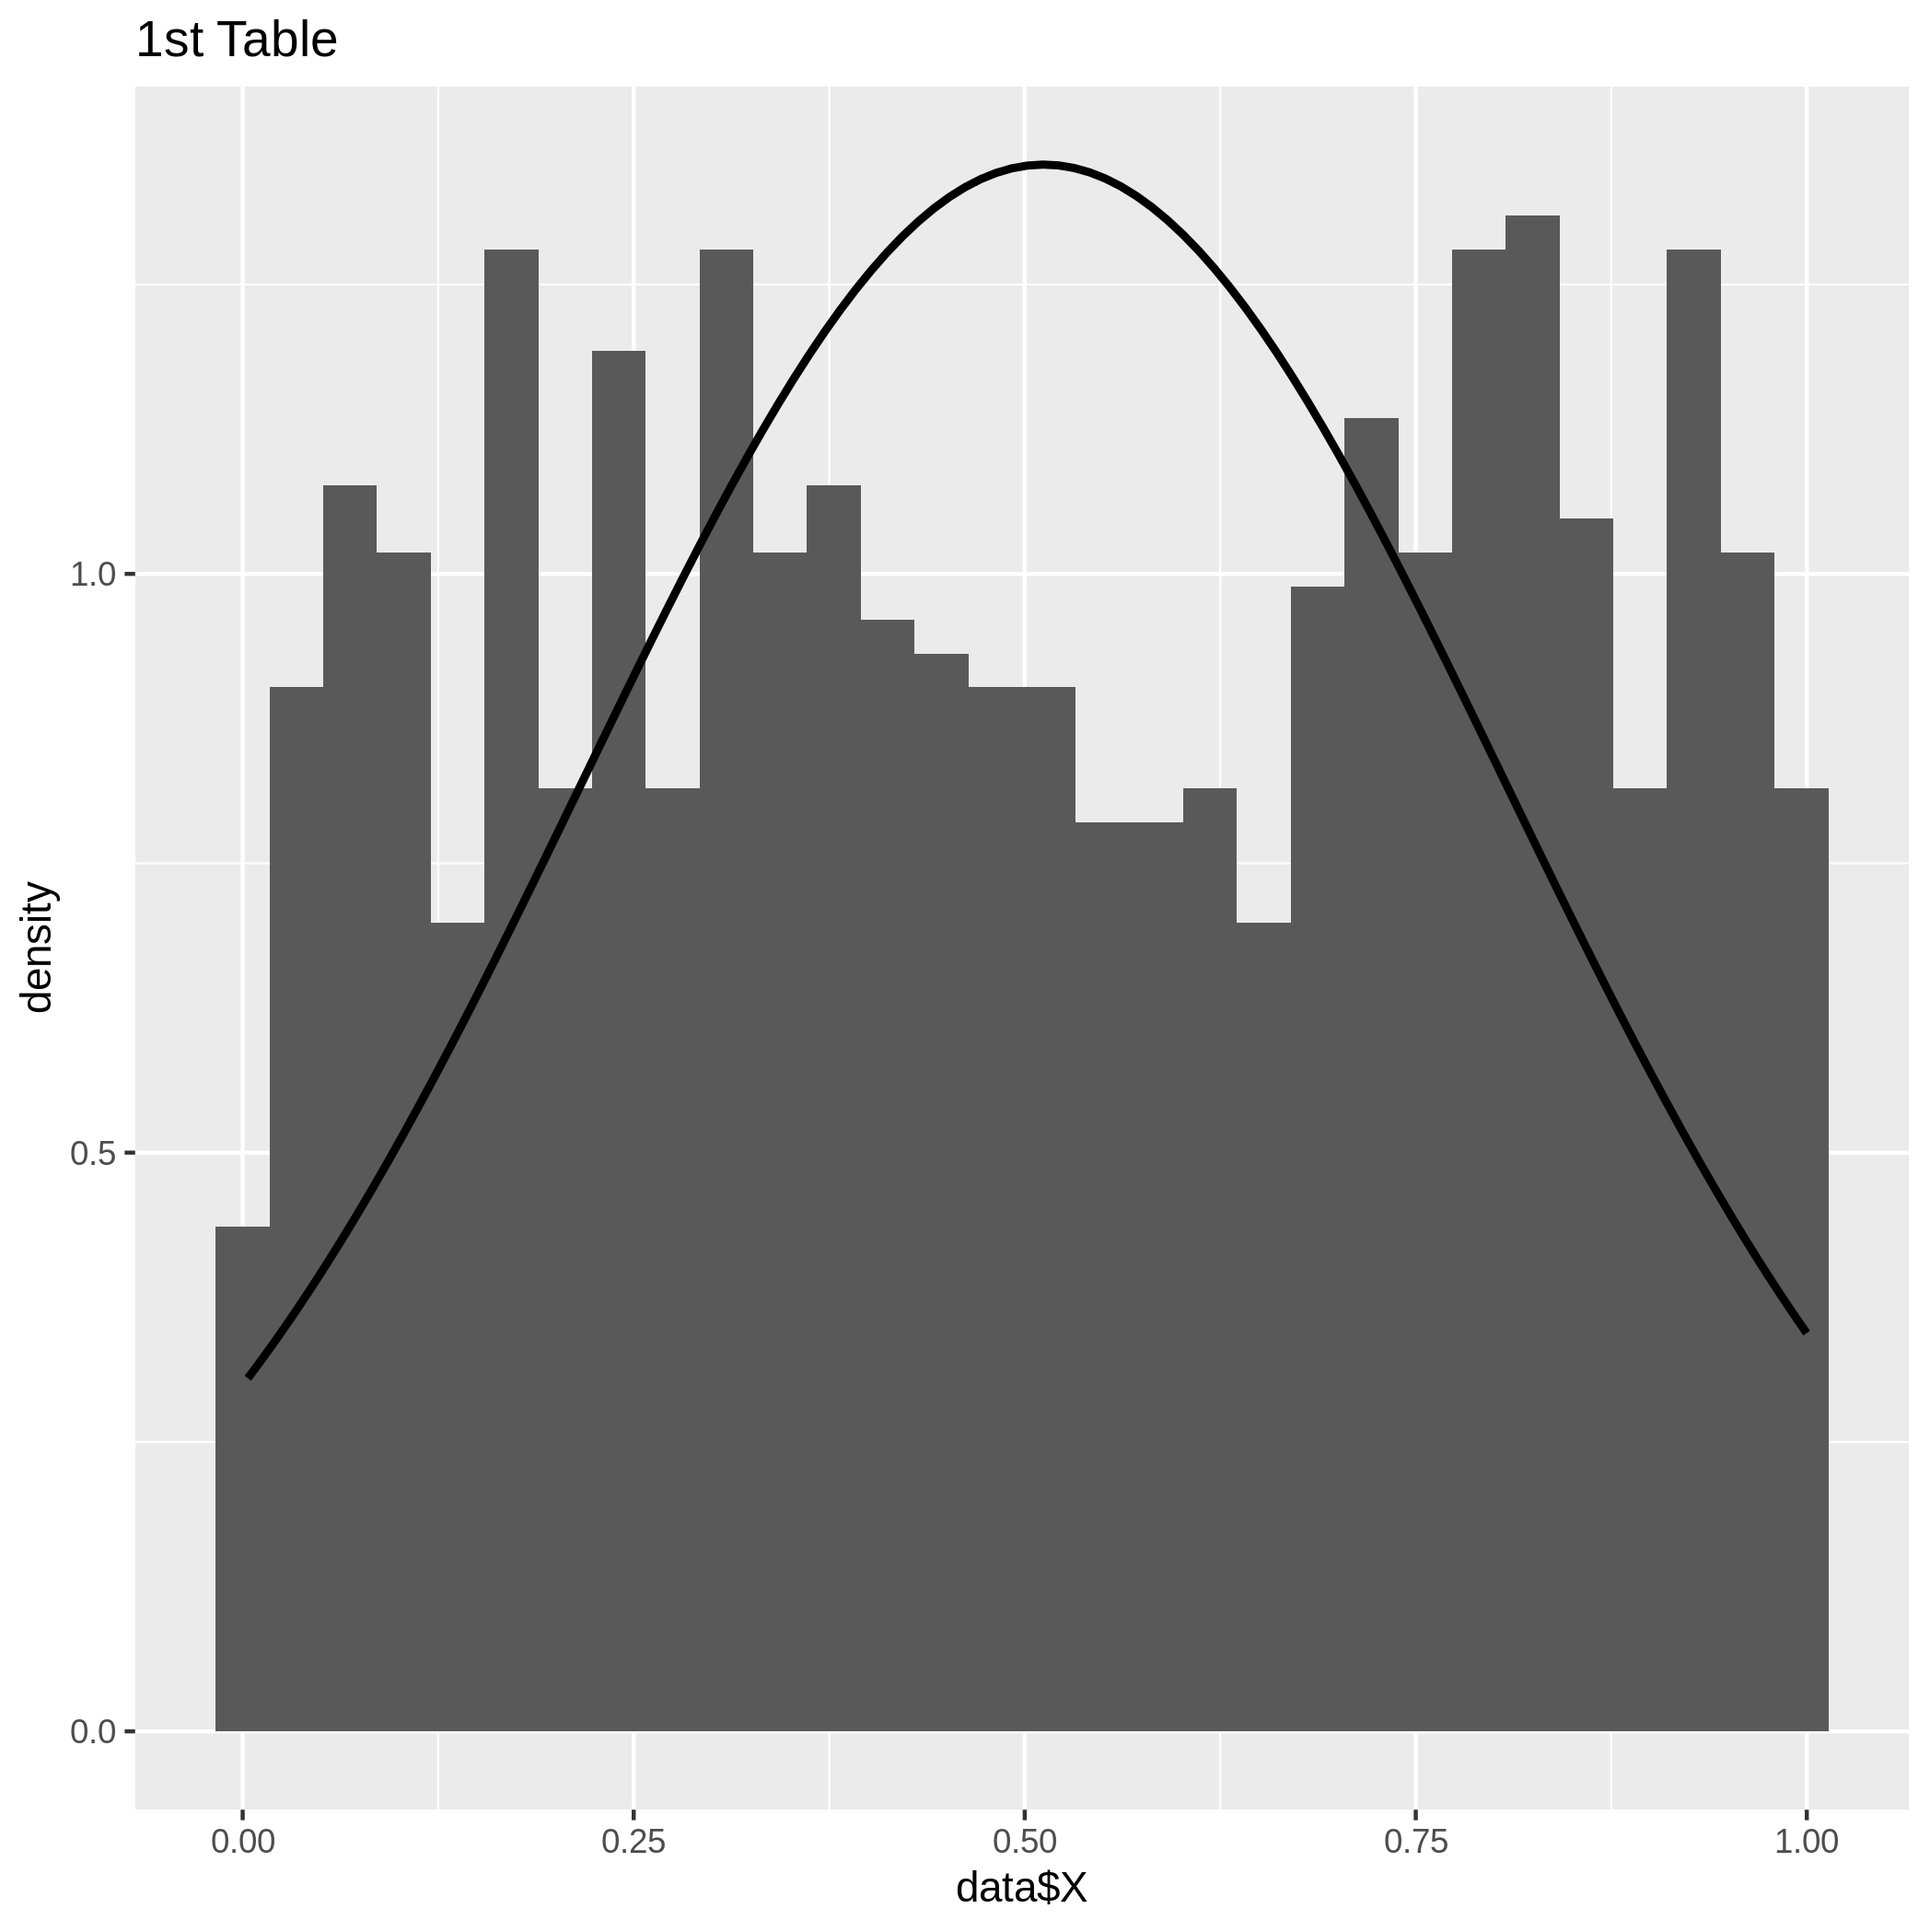
\includegraphics[width=6cm]{Table_1_histogram.png}}
				\hfill
				\subfigure[qqplot for table 1]{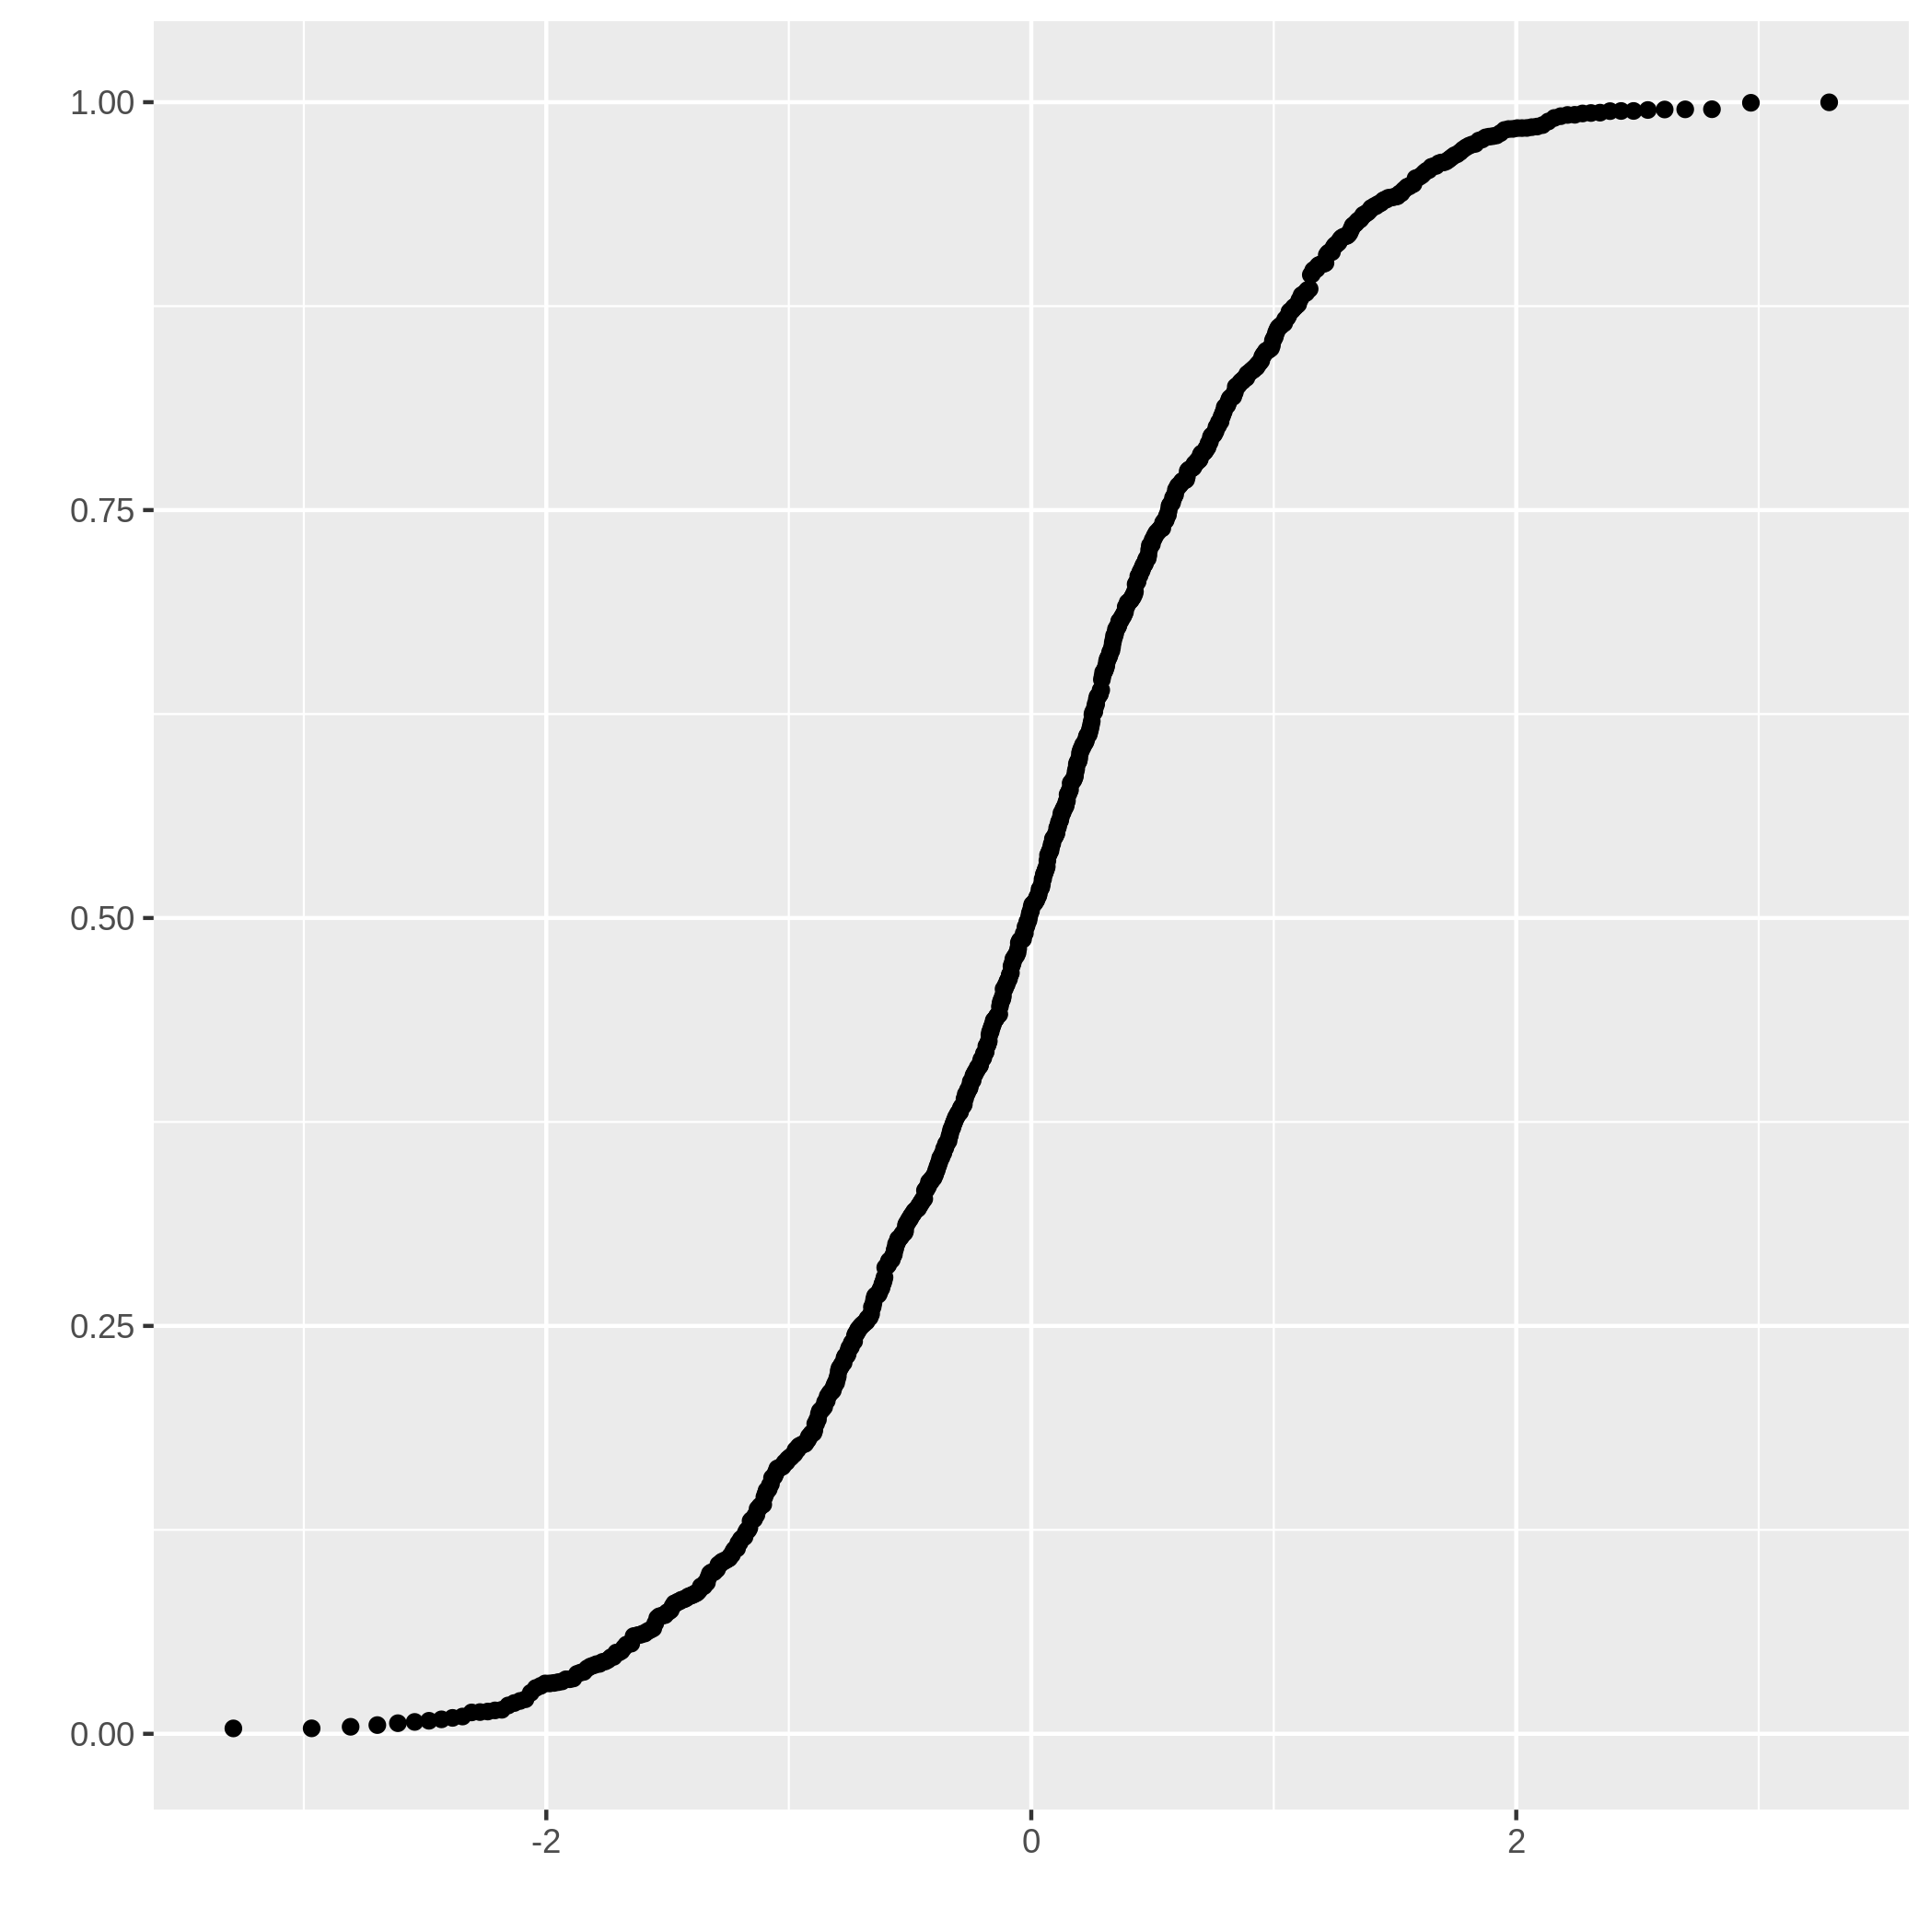
\includegraphics[width=6cm]{Table_1_qqplot.png}}
				\hfill
				\caption{Table1}
			\end{figure}
			\begin{figure}[H]
				\hfill
				\subfigure[Histogram for table 2]{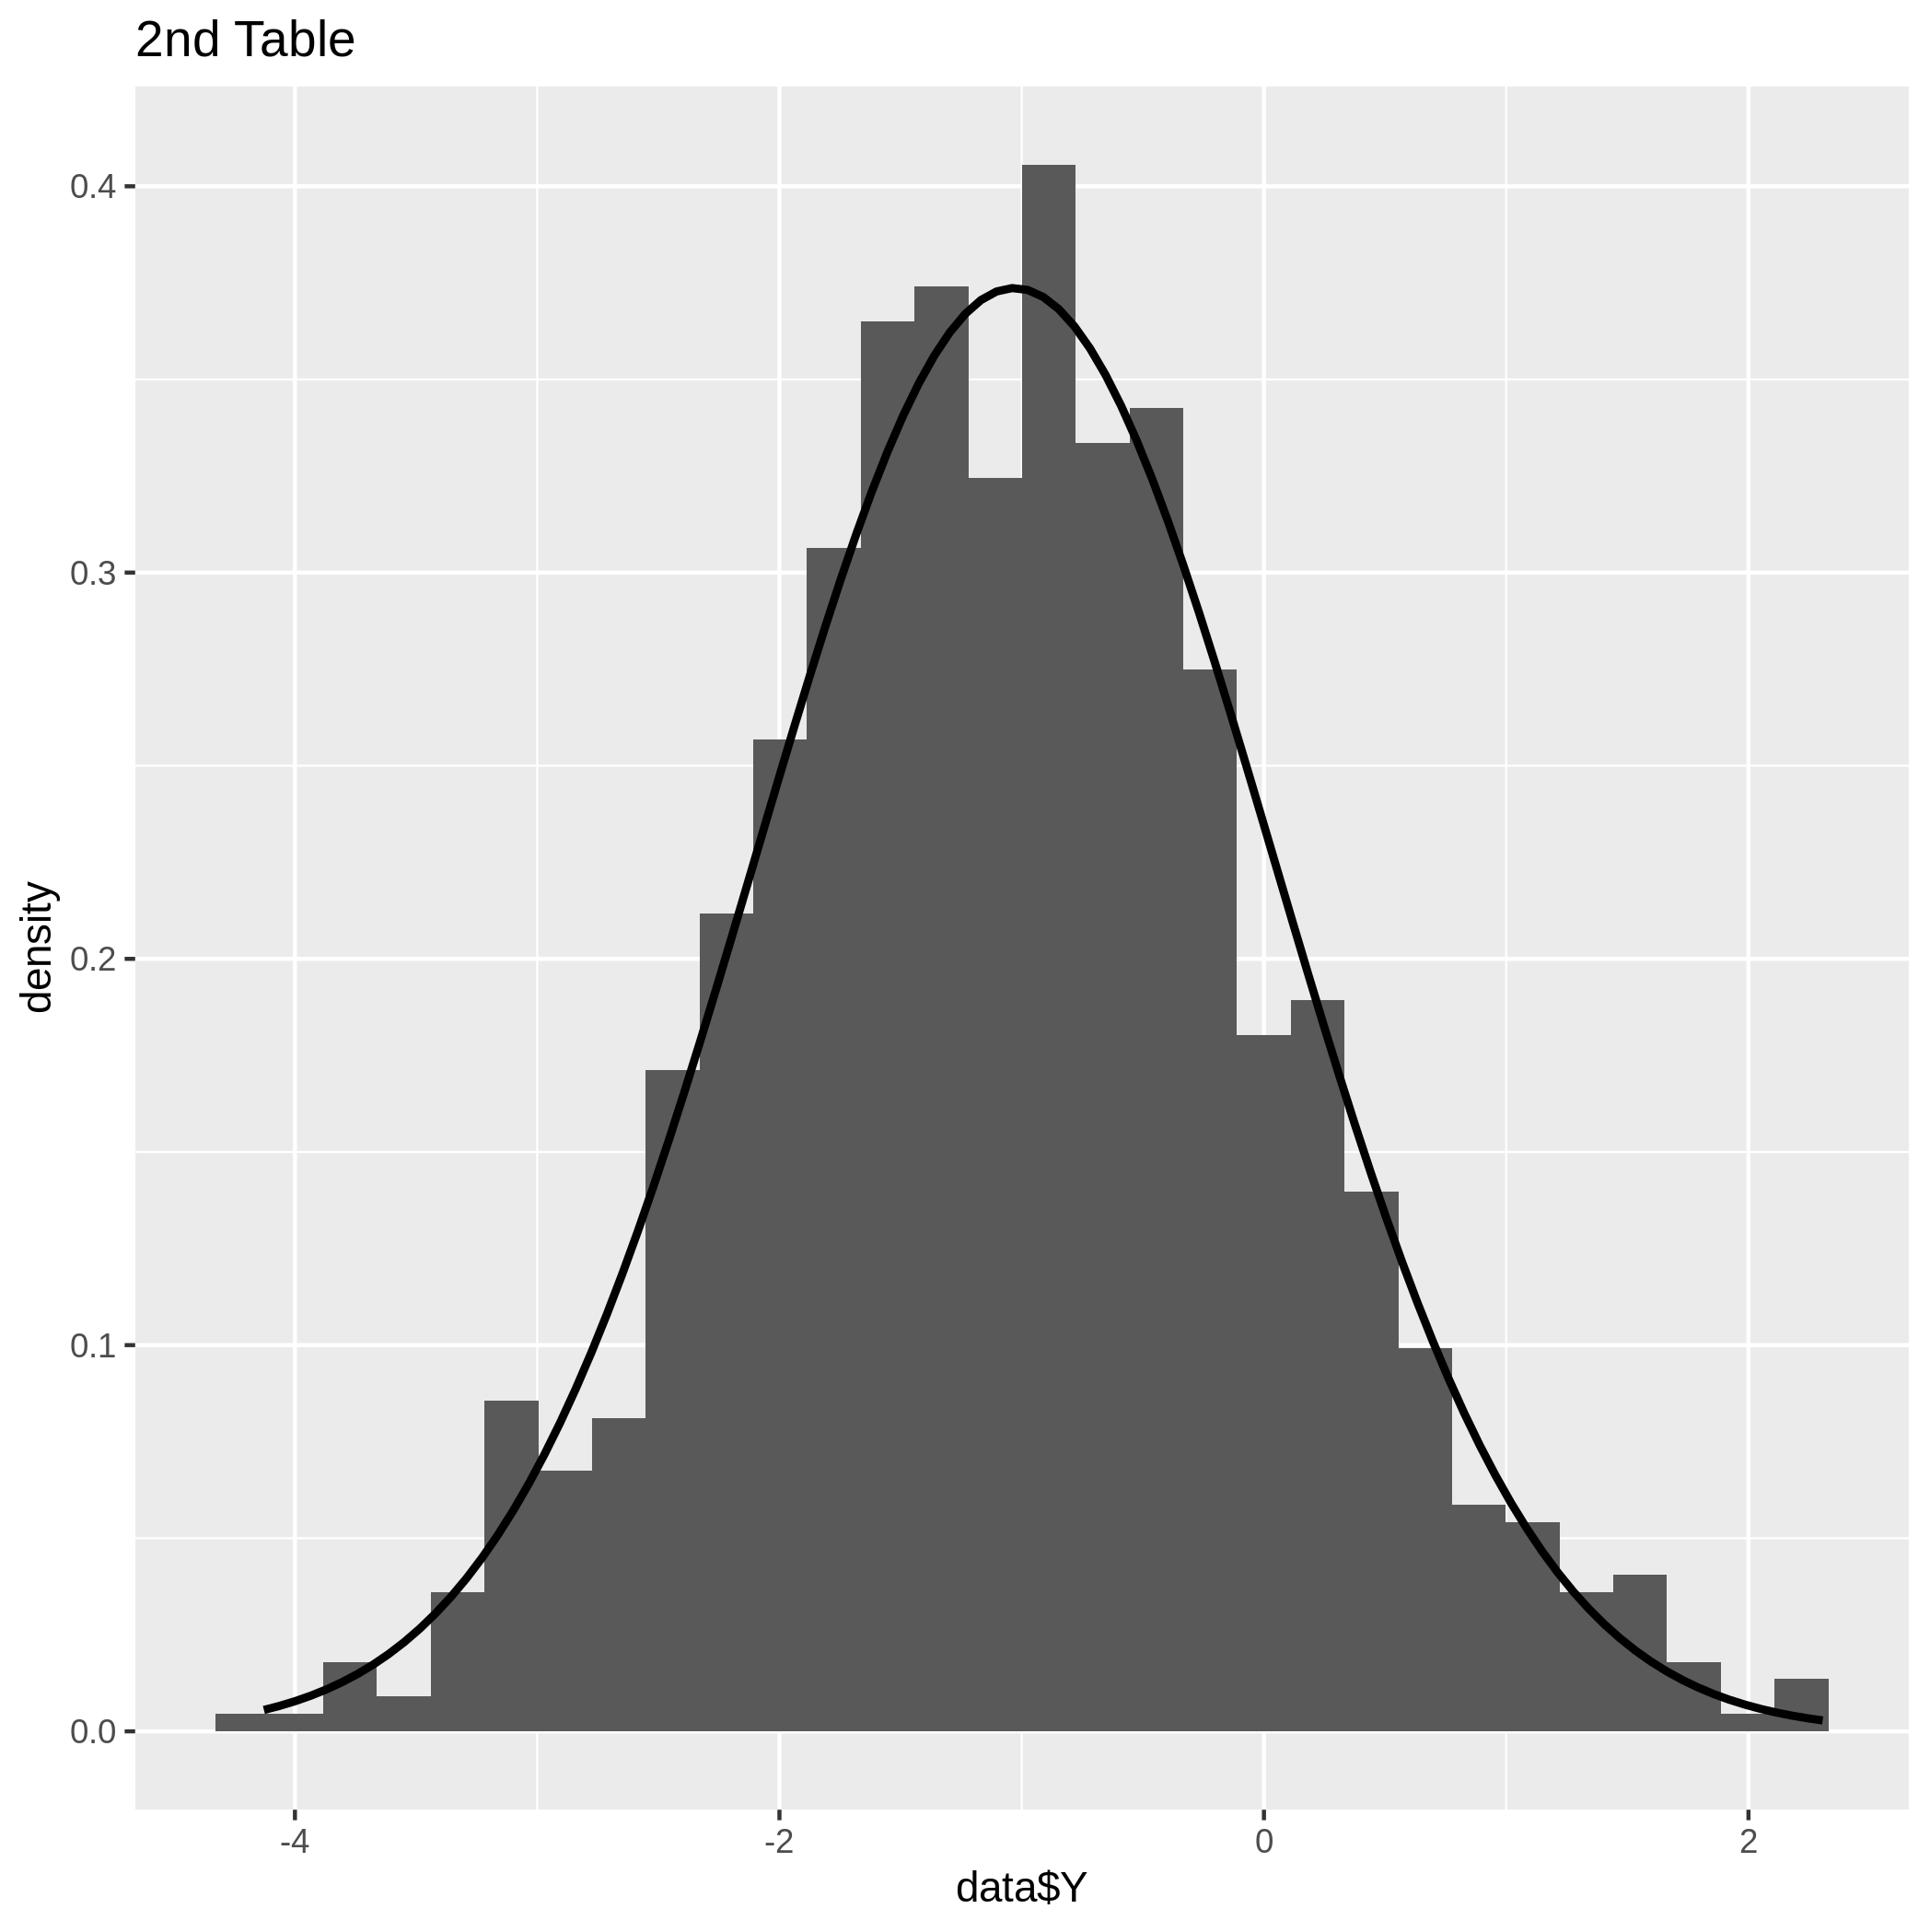
\includegraphics[width=6cm]{Table_2_histogram.png}}
				\hfill
				\subfigure[qqplot for table 2]{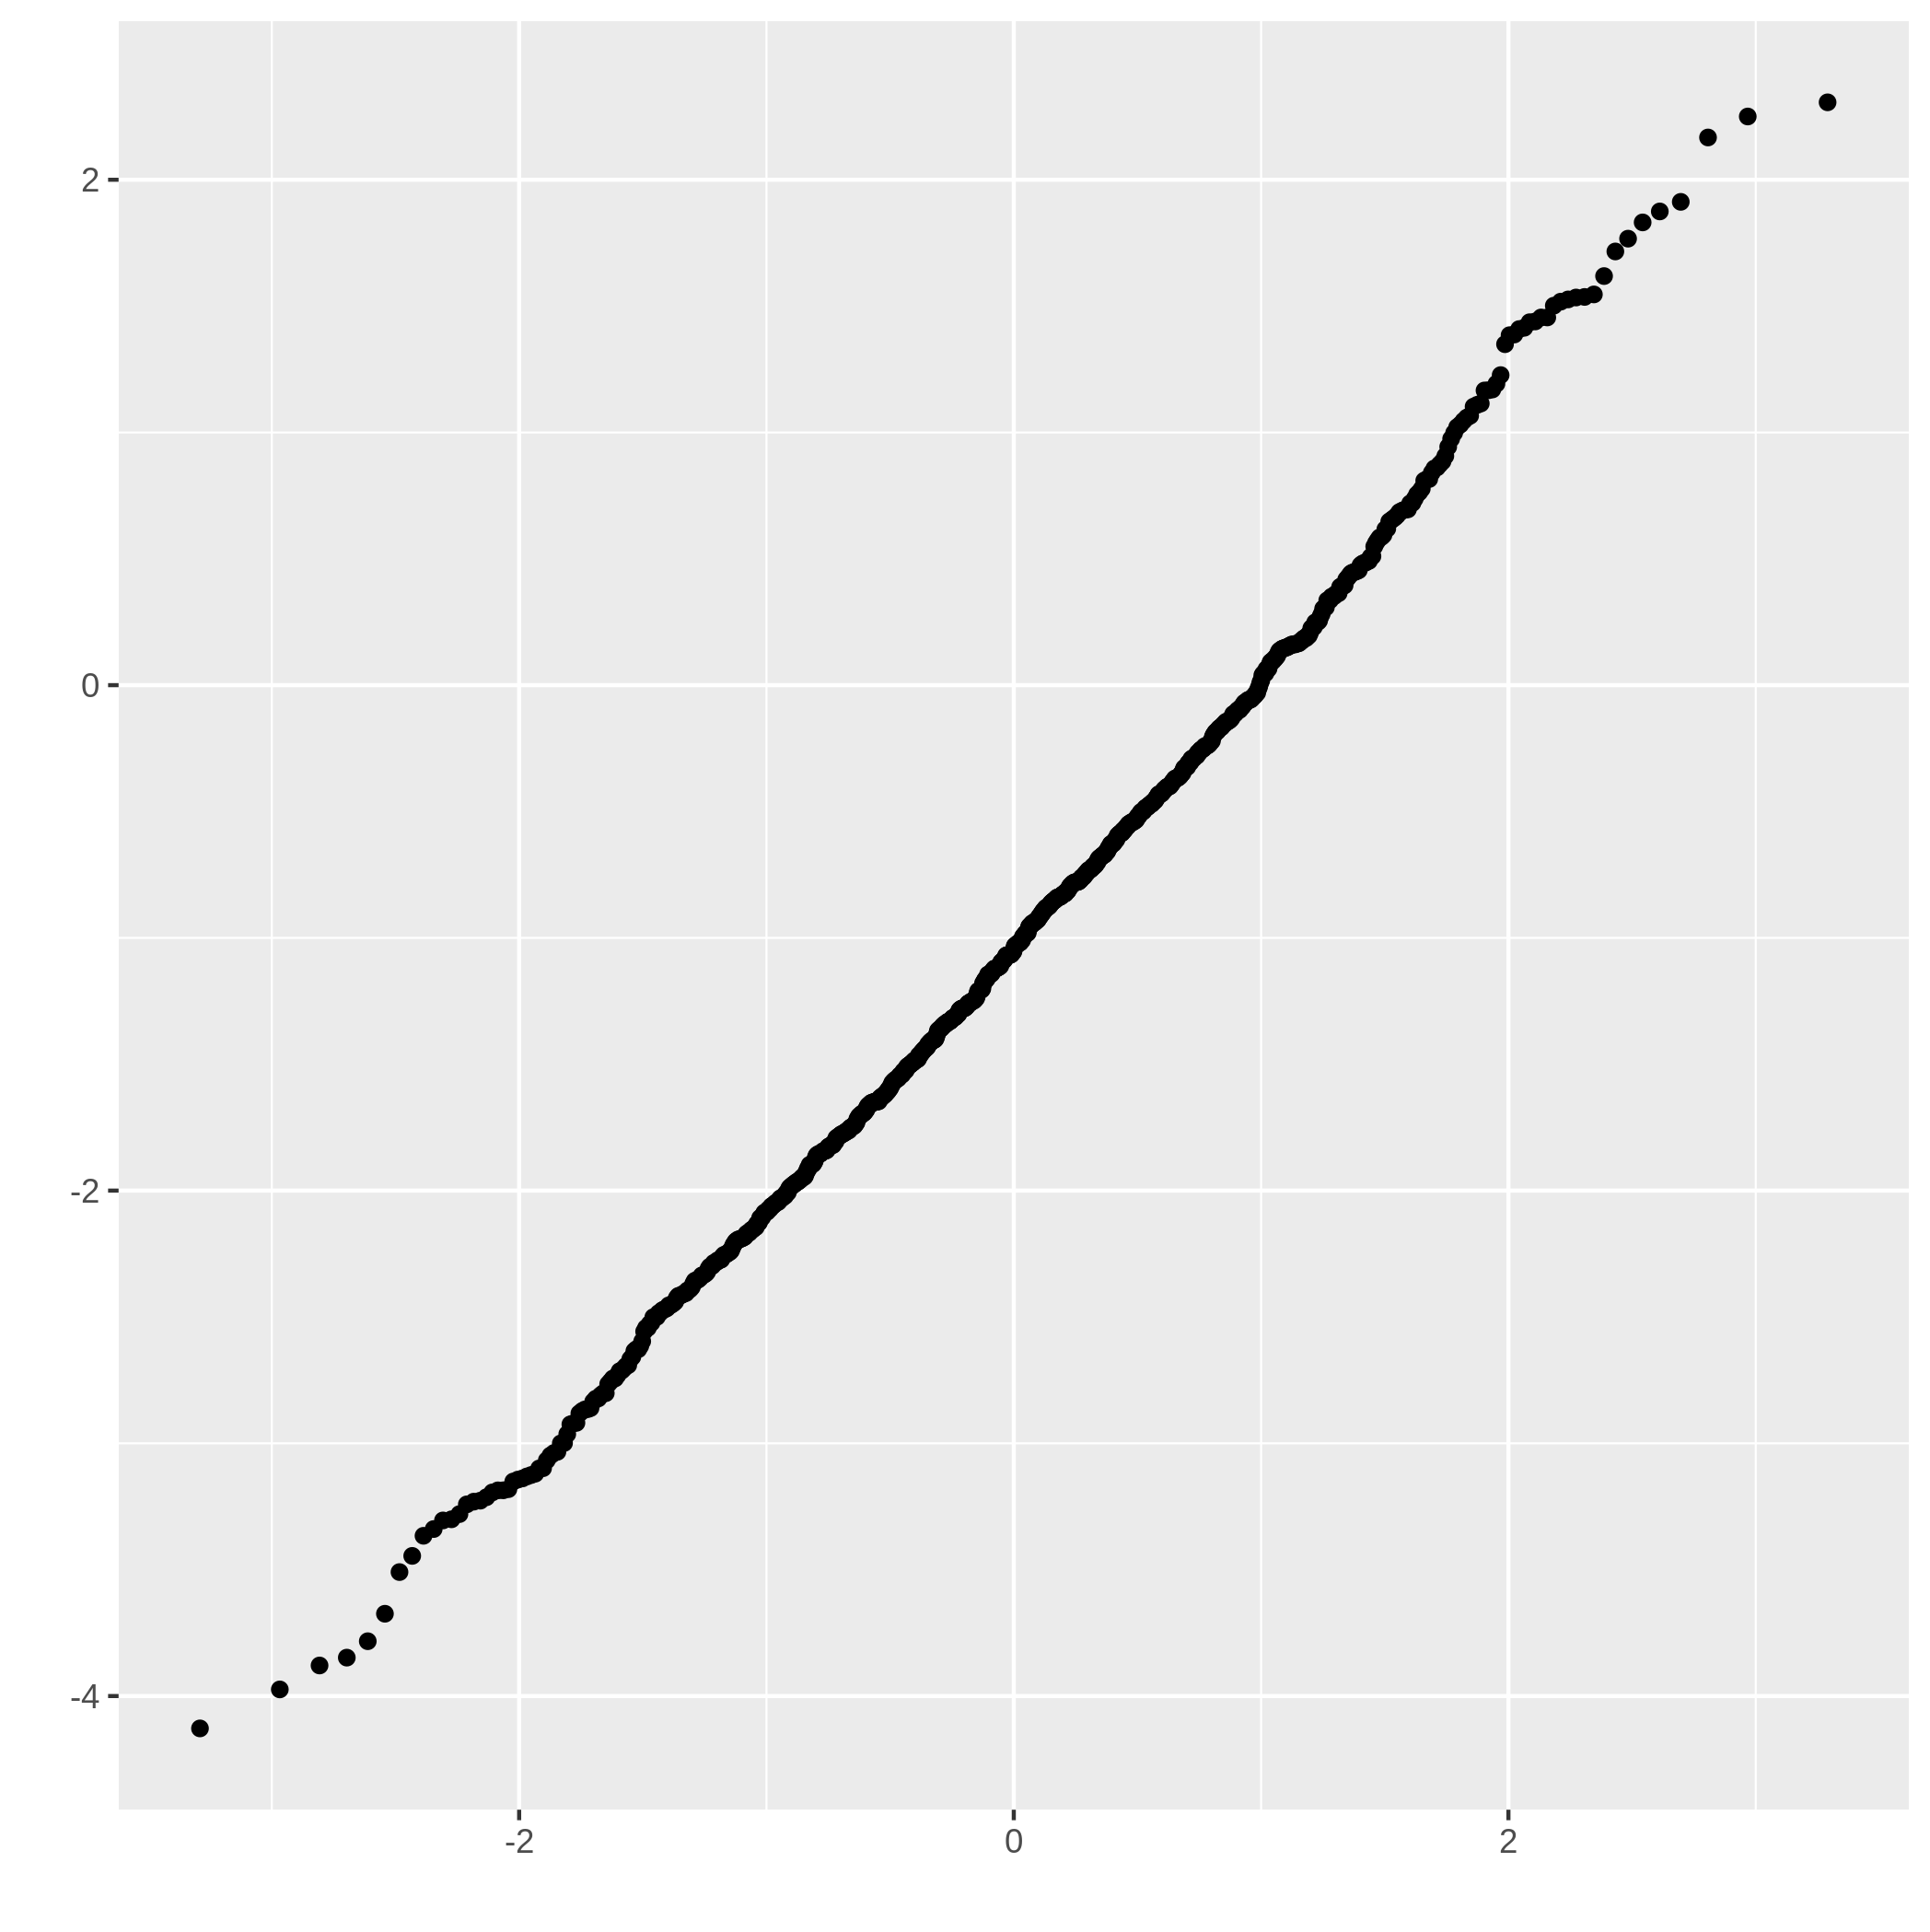
\includegraphics[width=6cm]{Table_2_qqplot.png}}
				\hfill
				\caption{Table2}
			\end{figure}
			\begin{figure}[H]
				\hfill
				\subfigure[Histogram for table 3]{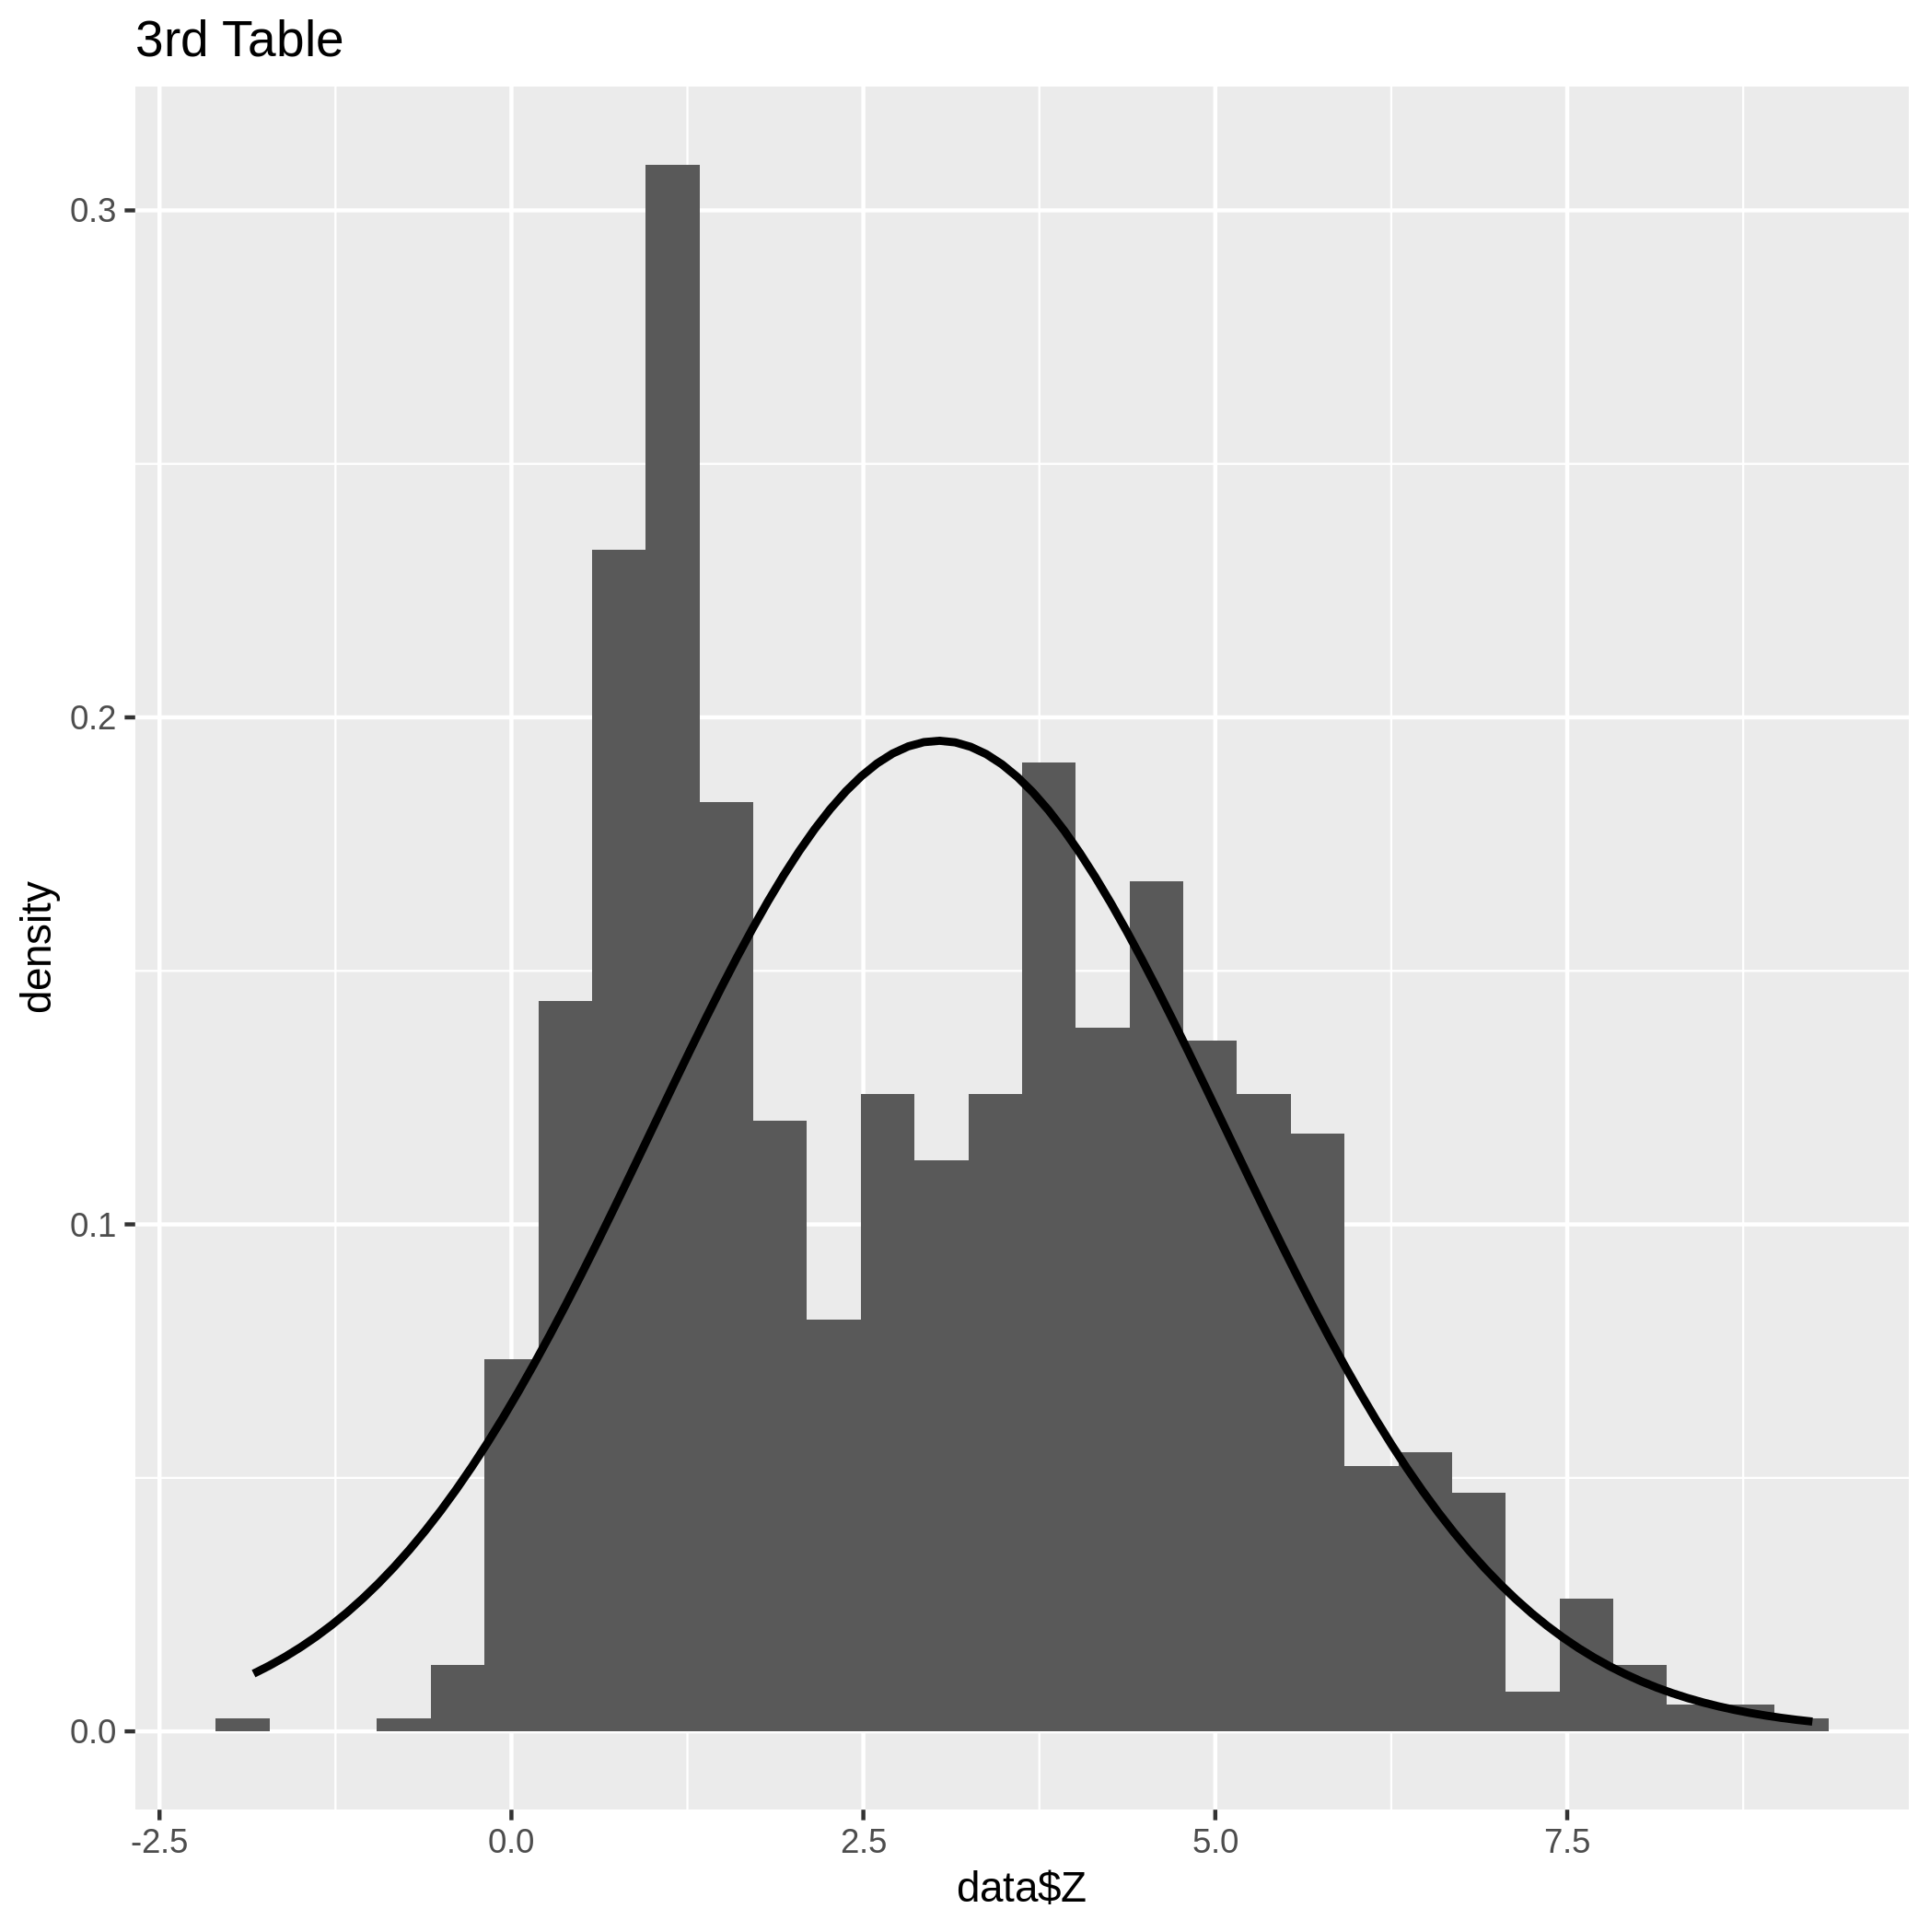
\includegraphics[width=6cm]{Table_3_histogram.png}}
				\hfill
				\subfigure[qqplot for table 3]{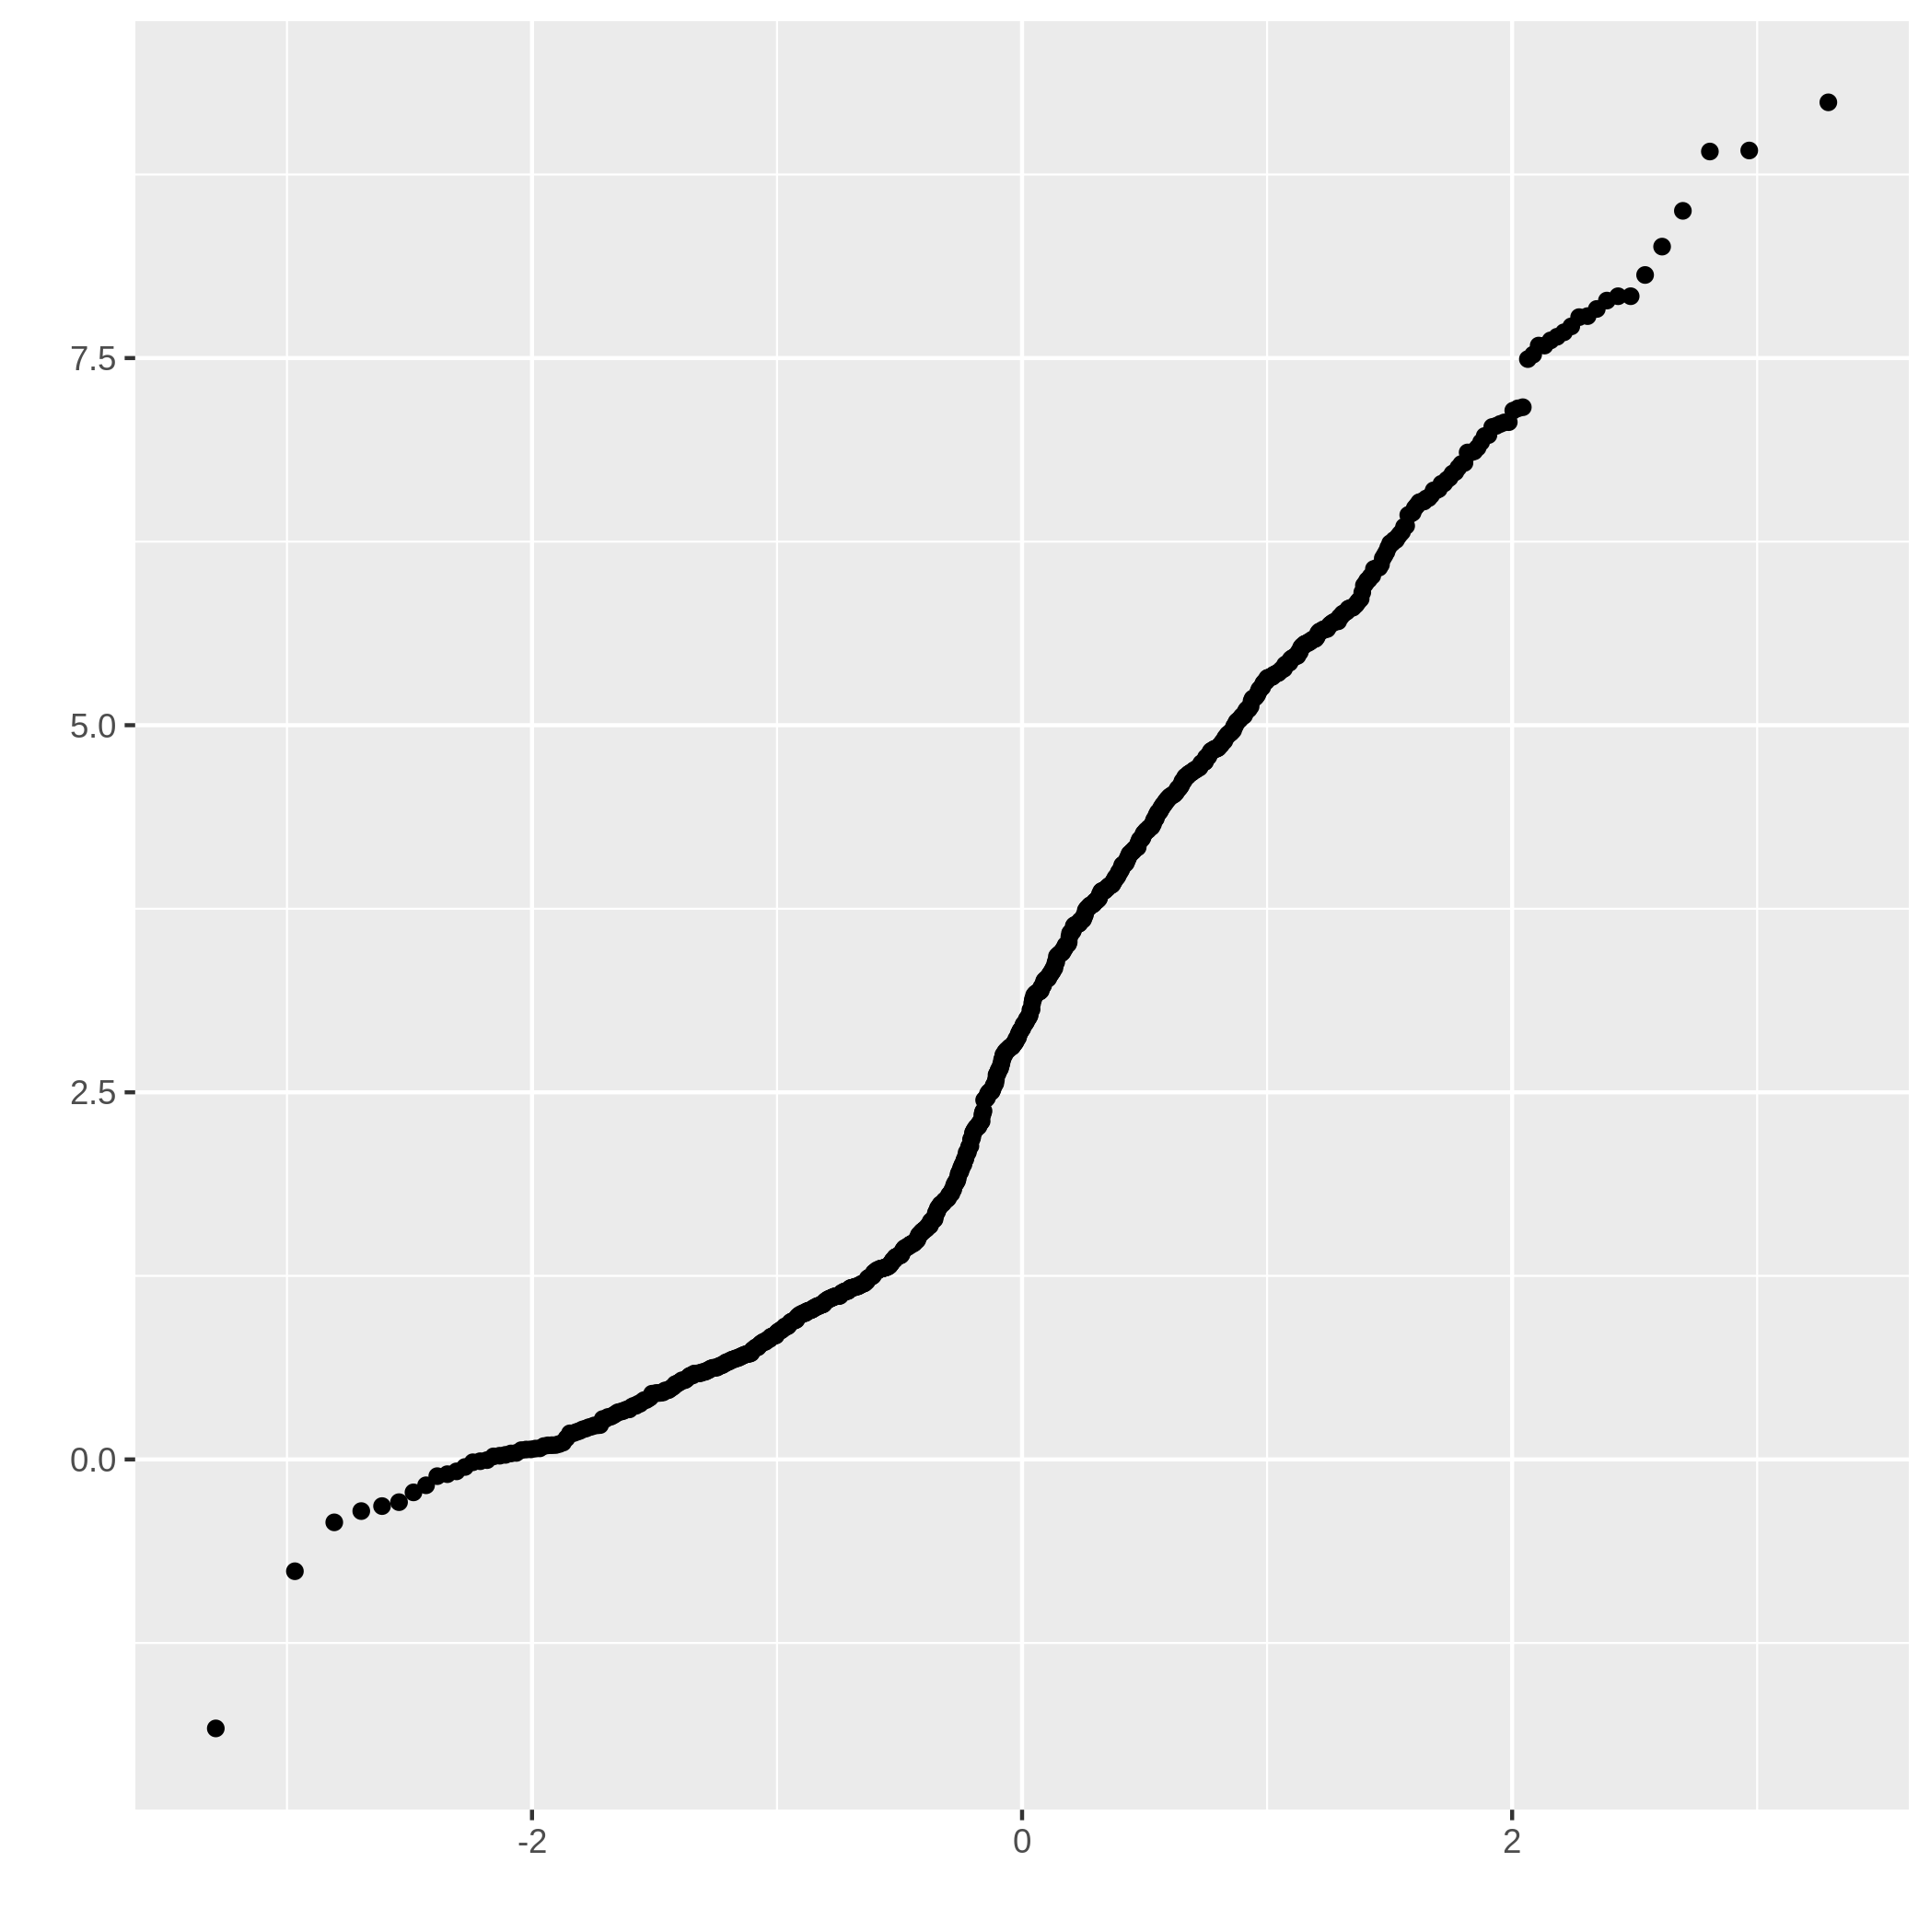
\includegraphics[width=6cm]{Table_3_qqplot.png}}
				\hfill
				\caption{Table3}
			\end{figure}
			
			From a visual point of view, we can see that only table 2 seems to have a normal distribution with a large number of people centered in the middle(Figure 2.a). This observation can be confirmed when looking at Figure 1.b. There we can observe that all the points are close to the first diagonal which is not the case in Figures 1.b and 3.b.
			Table 1 does not seem normal because on Figure 1.a, we can see a large number of people on the left and on the right with fewer people in the middle.
			Table 3 does not seem normal because on Figure 3.a we can see a succession of large number of people and small number of people going from left to right with some outliers on the left side. 
			
		\subsection{Skews and kurtosis}
			We used the function \textit{stat.desc()} from the \textit{"pastecs"} package to generate the following table:\\\\
			\begin{figure}[H]
				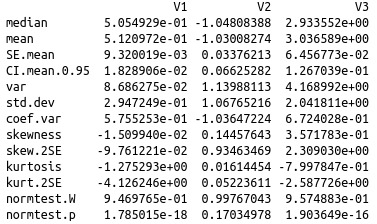
\includegraphics[width=12cm]{stat-desc.png}
				\caption{}
			\end{figure}
		
		From the table above (Figure 4.), we can see that the values of \textit{skew.2SE} and \textit{kurt.2SE} are either less or greater than 1 for tables 1 and 3 which means that the populations of those two tables have a significant skew and kurtosis. Those values are between -1 and 1 for table 2 which indicates normality in the population distribution.
		Figure.4 contains other important information such as the median, the mean and the standard deviation of the 3 populations but also the Shapiro-Wilk test for normality.	
				
		\subsection{Parametric test}
			We performed a Shapiro-Wilk test on the data sets to search for normality and we obtained the following:
			\begin{itemize}
				\item table 1: W = 0.94698, p-value \textless{}  2.2e-16
				\item table 2: W = 0.99767, p-value = 0.1703
				\item table 3: W = 0.95749, p-value \textless{}  2.2e-16
			\end{itemize} 
		
			As we can see from the results above, only table 2 has a p-value greater than 0.05 which indicate a normal distribution within its population. On the other hand, a p-value \textless{} 0.5 for tables 1 and table 3 indicates an absence of normality.
		\section {Correcting the data}
			\subsection{Remove the outliers in table 3}
				As  we can see on Figure 3.a above, some outliers can be spotted on the left. So we looked at the data and observed that only 15 out of 100 entries have negative values. So, we removed those values and performed the Shapiro-Wilk test again and we obtained the following:\\
				
				W = 0.95088, p-value \textless{} 2.2e-16 \\
				which is not much different from what we got in section 2.3
			\subsection{Log transformation}
				We performed a log transformation on tables 1 and 3, then ran the Shapiro-Wilk test again and obtained the following:
				\begin{itemize}
					\item table 1: W = 0.83531, p-value \textless{}  2.2e-16,
					\item table 2: W = 0.89799, p-value \textless{}  2.2e-16.
				\end{itemize} 
				As we can see the p-value didn't improve from what we got in section 2.3. So the log transformation is not efficient for both cases.
			\subsection{Log(table + 1) transformation}
				We performed another log transformation on tables 1 and 3 (but this time we added 1 to the old values before applying the log), then we ran the Shapiro-Wilk test again and obtained the following:
				\begin{itemize}
					\item table 1: W = 0.94421, p-value \textless{}  2.2e-16
					\item table 2: W = 0.95601, p-value \textless{}  2.2e-16
				\end{itemize} 
			\subsection{Square root transformation}
				We performed a square root transformation on tables 1 and 3 then  ran the Shapiro-Wilk test again and obtained the following:
				\begin{itemize}
					\item table 1: W = 0.83531, p-value \textless{}  2.2e-16
					\item table 2: W = 0.89799, p-value \textless{}  2.2e-16
				\end{itemize} 
			\subsection{Reciprocal Transformation}
				We performed a reciprocal transformation on tables 1 and 3 then ran the Shapiro-Wilk test again and obtained the following:
				\begin{itemize}
					\item table 1: W = 0.93084, p-value \textless{}  2.2e-16
					\item table 2: W = 0.71248, p-value \textless{}  2.2e-16
				\end{itemize} 
		\section{conclusion}
			Out of the 3 tables we obtained for this experiment, only the second table appeared to be normally distributed. This conclusion comes from observing the histograms and qqplots of the tables, by computing their skews and kurtosis and by performing a Shapiro-Wilk test for normality on them. We tried to correct the data contained in tables 1 and 3 by using techniques such as eliminating outliers, log transformations and square root transformations. However, none of these techniques worked as we can see in the previous section. The P-values returned by the Shapiro-Wilk test on the new data is not different from what we obtained for the original tables. Therefore, since parametric test didn't work for tables 1 and 3, the next step is to perform non-parametric test on them and see what we obtain. 
		\section{Libraries used}
			During the experimentation, we considered using the following packages,
			\begin{itemize}
				\item \textit{"ggplot2"} to draw the histograms and the qqplots,
				\item \textit{"pastecs"} to generate the table in section 2.2 by using its \textit{stat.desc()} function. 
			\end{itemize}
		
			
	
	
\end{document}